\documentclass{article}

\usepackage{graphicx}
\usepackage{tikz}
\usepackage{tikzsymbols}
\usetikzlibrary{calc,patterns,shapes.geometric}
\pagestyle{empty}
\usepackage[margin=0pt]{geometry}
\geometry{papersize={14in,12in}}

\def\centerarc[#1](#2)(#3:#4:#5){\draw[#1] ($(#2)+({#5*cos(#3)},{#5*sin(#3)})$) arc (#3:#4:#5);}

\begin{document}
	\begin{figure}
		\centering
		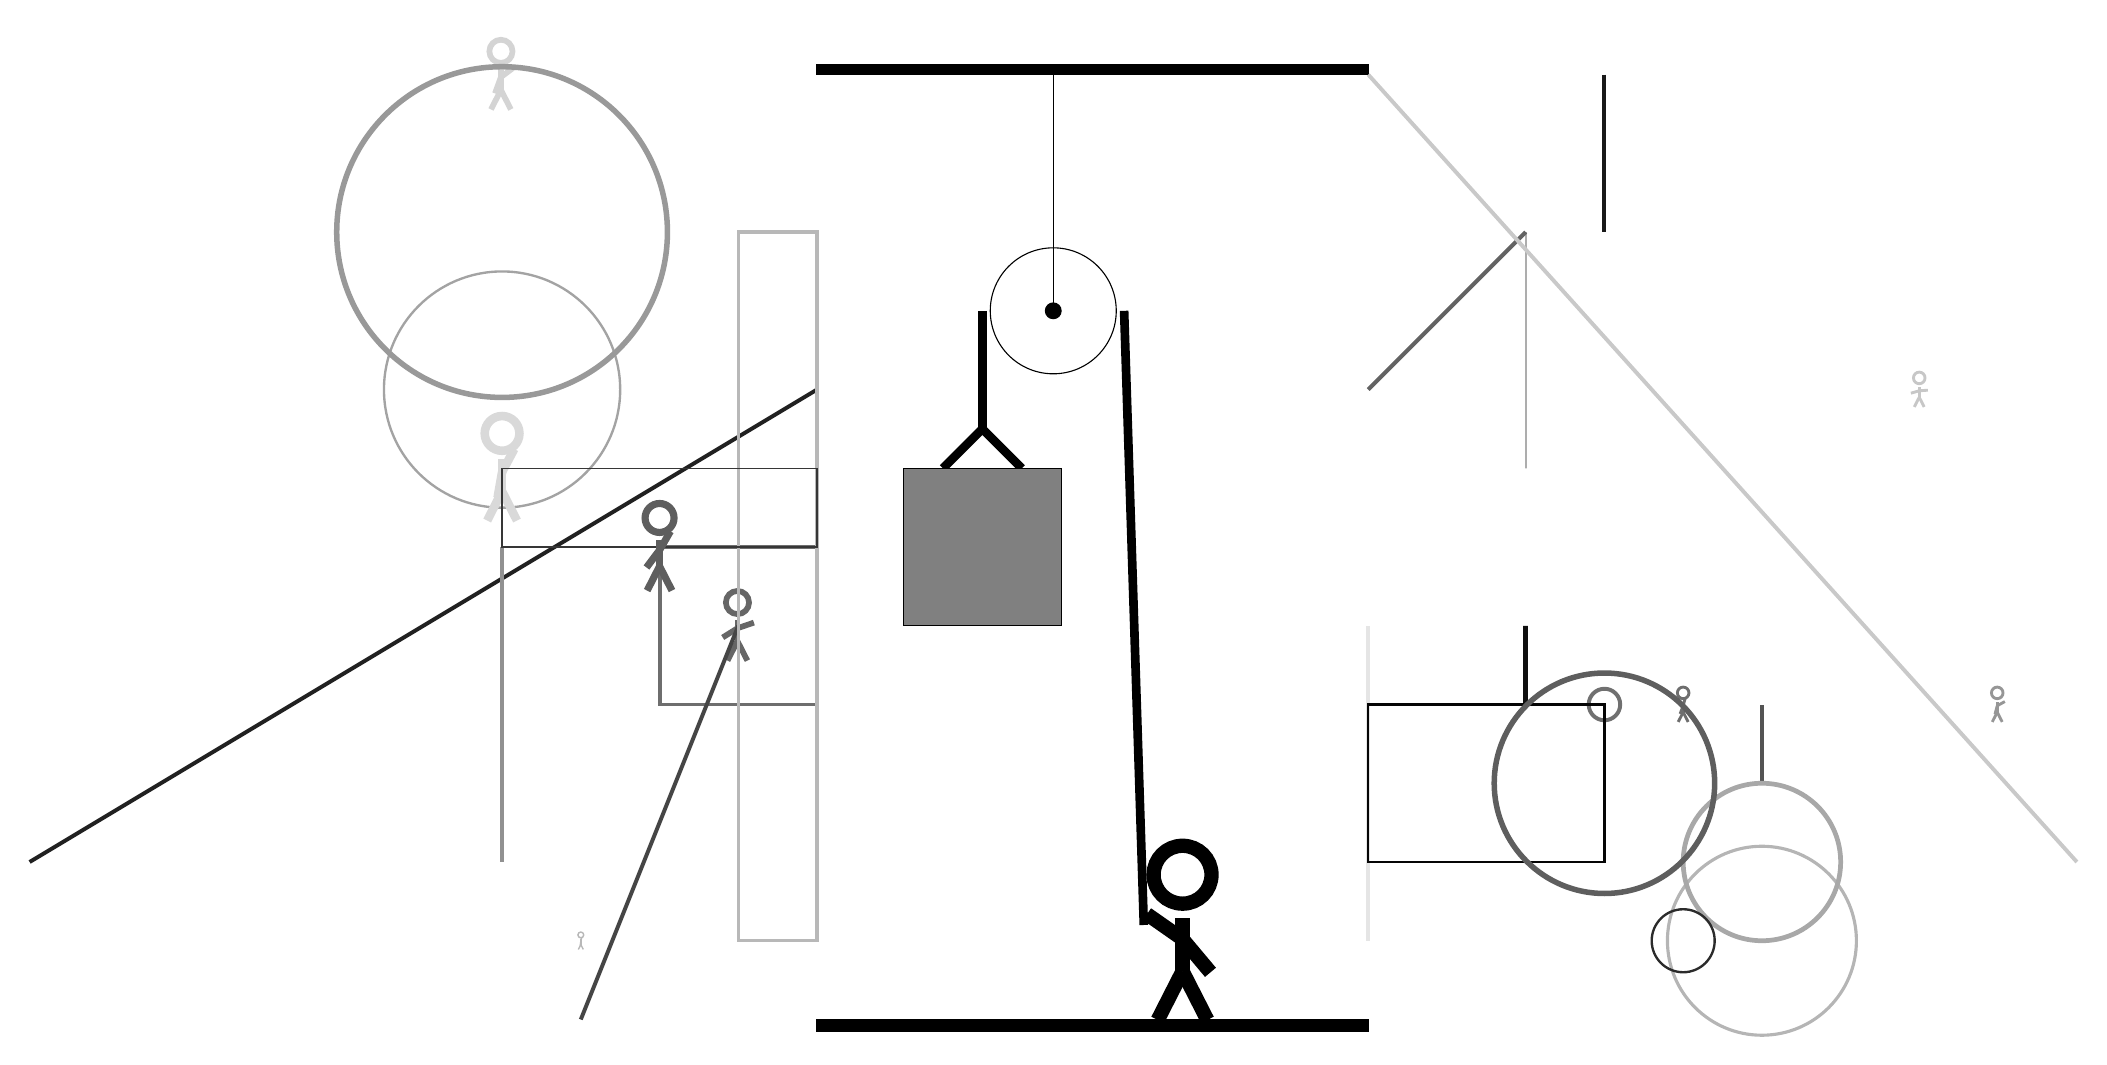
\begin{tikzpicture}
			%%%%% START %%%%%
			
			\draw[fill=black] (-2, 9) rectangle (5, 9.125);
			
			\draw (1, 6) circle (0.8);
			\draw[fill=black] (1, 6) circle (0.1);
			\draw (1, 9) -- (1, 6);
			
			\node[line width=0.3mm, color=black!41] at (13, 1) {\Strichmaxerl[2][75][29]};
			
			\node[line width=0.4mm, color=black!60] at (-3, 2) {\Strichmaxerl[4][32][19]};
			\draw[line width=0.5mm, color=black!87](-2, 5) -- (-12, -1);
			\draw[line width=0.5mm, color=black!43](-6, 3) -- (-6, -1);
			\node[line width=0.6mm, color=black!17] at (-6, 9) {\Strichmaxerl[4][70][37]};
			\draw[line width=0.2mm, color=black!32] (7, 7) rectangle (7, 4);
			
			\node[line width=0.7mm, color=black!22] at (12, 5) {\Strichmaxerl[2][16][4]};
			
			\draw[line width=0.5mm, color=black!34](-2, 4) -- (-2, -2);
			\draw[line width=0.5mm, color=black!57] (-2, 3) rectangle (-4, 1);
			\node[line width=0.7mm, color=black!28] at (-5, -2) {\Strichmaxerl[1][82][77]};
			
			\draw[line width=0.7mm, color=black!94] (7, 2) rectangle (7, 1);
			\draw[line width=0.5mm, color=black!61](7, 7) -- (5, 5);
			\draw[line width=0.5mm, color=black!21](5, 9) -- (14, -1);
			
			\draw[line width=0.5mm, color=black!73](-3, 2) -- (-5, -3);
			\node[line width=0.6mm, color=black!57] at (9, 1) {\Strichmaxerl[2][69][75]};
			\draw[line width=0.4mm, color=black!28] (-2, -2) rectangle (-3, 7);
			
			\draw [line width=0.5mm, color=black!56](8, 1) circle (0.2);
			
			\draw[line width=0.5mm, color=black!10](5, -2) -- (5, 2);
			\draw [line width=0.3mm, color=black!36](-6, 5) circle (1.5);
			\draw [line width=0.4mm, color=black!29](10, -2) circle (1.2);
			\node[line width=0.4mm, color=black!15] at (-6, 4) {\Strichmaxerl[6][80][62]};
			
			\draw[line width=0.5mm, color=black!67](10, 0) -- (10, 1);
			\draw[line width=0.2mm, color=black!79] (-2, 3) rectangle (-6, 4);
			\draw [line width=0.7mm, color=black!40](-6, 7) circle (2.1);
			\draw[line width=0.3mm, color=black!98] (5, -1) rectangle (8, 1);
			
			\draw [line width=0.6mm, color=black!34](10, -1) circle (1.0);
			
			\draw[line width=0.5mm, color=black!90](8, 9) -- (8, 7);
			\draw [line width=0.2mm, color=black!42](9, 3) circle (0.0);
			\draw [line width=0.3mm, color=black!83](9, -2) circle (0.4);
			\draw [line width=0.7mm, color=black!63](8, 0) circle (1.4);
			\node[line width=0.4mm, color=black!63] at (-4, 3) {\Strichmaxerl[5][53][60]};
			
			\draw[line width=1.1mm] (-0.4, 4.0) -- (0.1, 4.5) -- (0.6, 4.0);
			\draw[fill=black!50] (-0.9, 4.0) rectangle (1.1, 2.0);
			
			\draw[line width=1.1mm] (0.1, 6) -- (0.1, 4.5);
			\centerarc[line width=1.1mm](1, 6)(0:180:0.9);
			\draw[line width=1.1mm](1.9, 6) -- (2.15, -1.8);
			
			\node at (2.6, -1.9) {\Strichmaxerl[10][-35][-50]};
			
			\draw[fill=black] (-2, -3) rectangle (5, -3.15);
			
			%%%%% END %%%%%
		\end{tikzpicture}
	\end{figure}	
\end{document}